% Extracted from CollisionPaper main eccf65a46a62b77d8efd297bffc42181d5f69751; English source captions.
\documentclass[a4paper,11pt]{ltjsarticle}

\usepackage[haranoaji]{luatexja-preset}
\usepackage{amsmath}
\usepackage{amssymb}
\usepackage{booktabs}
\usepackage{float}
\usepackage{graphicx}
\usepackage{hyperref}
\usepackage{microtype}
\usepackage{siunitx}
\usepackage[margin=25mm]{geometry}
\usepackage{subcaption}
\usepackage{tikz}
\usetikzlibrary{arrows.meta,calc,positioning}
\usepackage{hhline}


\hypersetup{
  colorlinks=true,
  linkcolor=blue,
  citecolor=blue,
  urlcolor=blue
}


\renewcommand{\figurename}{Figure~}
\renewcommand{\tablename}{Table~}
\pagestyle{empty}
\makeatletter\@namedef{r@sec:collision_statistics}{{2.2}{1}{}{}{}}\@namedef{r@sec:synthetic_hologram_generation}{{4.5}{1}{}{}{}}\makeatother
% Citation number follows first-appearance order in the pinned main.tex (unsrt).
\makeatletter\@namedef{b@HoloD3}{45}\makeatother
\begin{document}
\setcounter{figure}{3}
\begin{figure}
  \centering
  \begin{minipage}
    {0.45\linewidth}
    \centering
    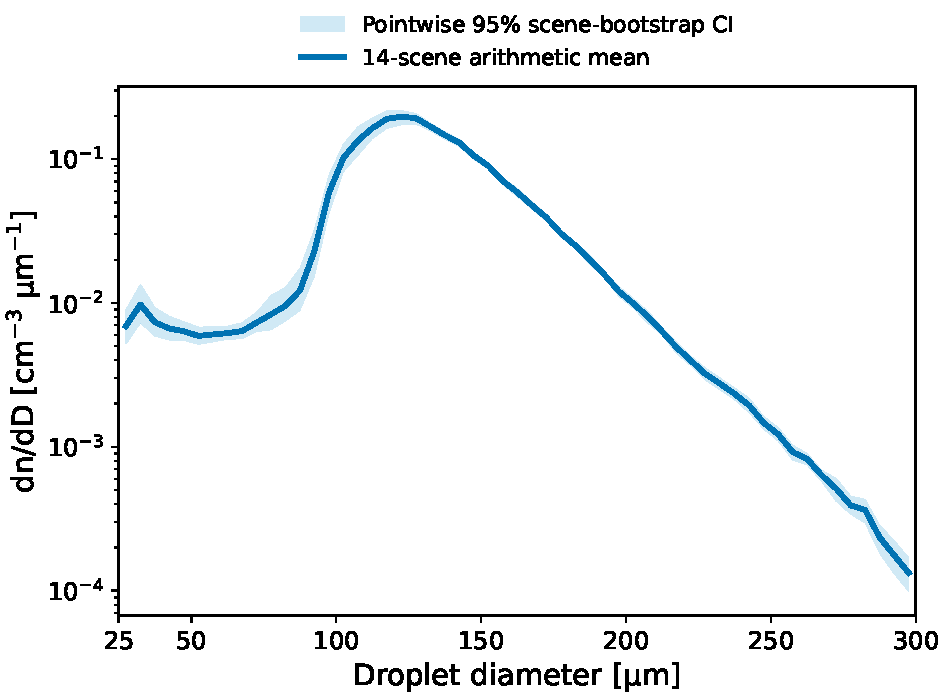
\includegraphics[width=0.98\linewidth]{figures/methods/particle_size_distribution_mean_ci_260715.pdf}
    \subcaption{
      Droplet number-density distribution
    }
  \end{minipage}
  \hspace{3mm}
  \begin{minipage}
    {0.48\linewidth}
    \centering
    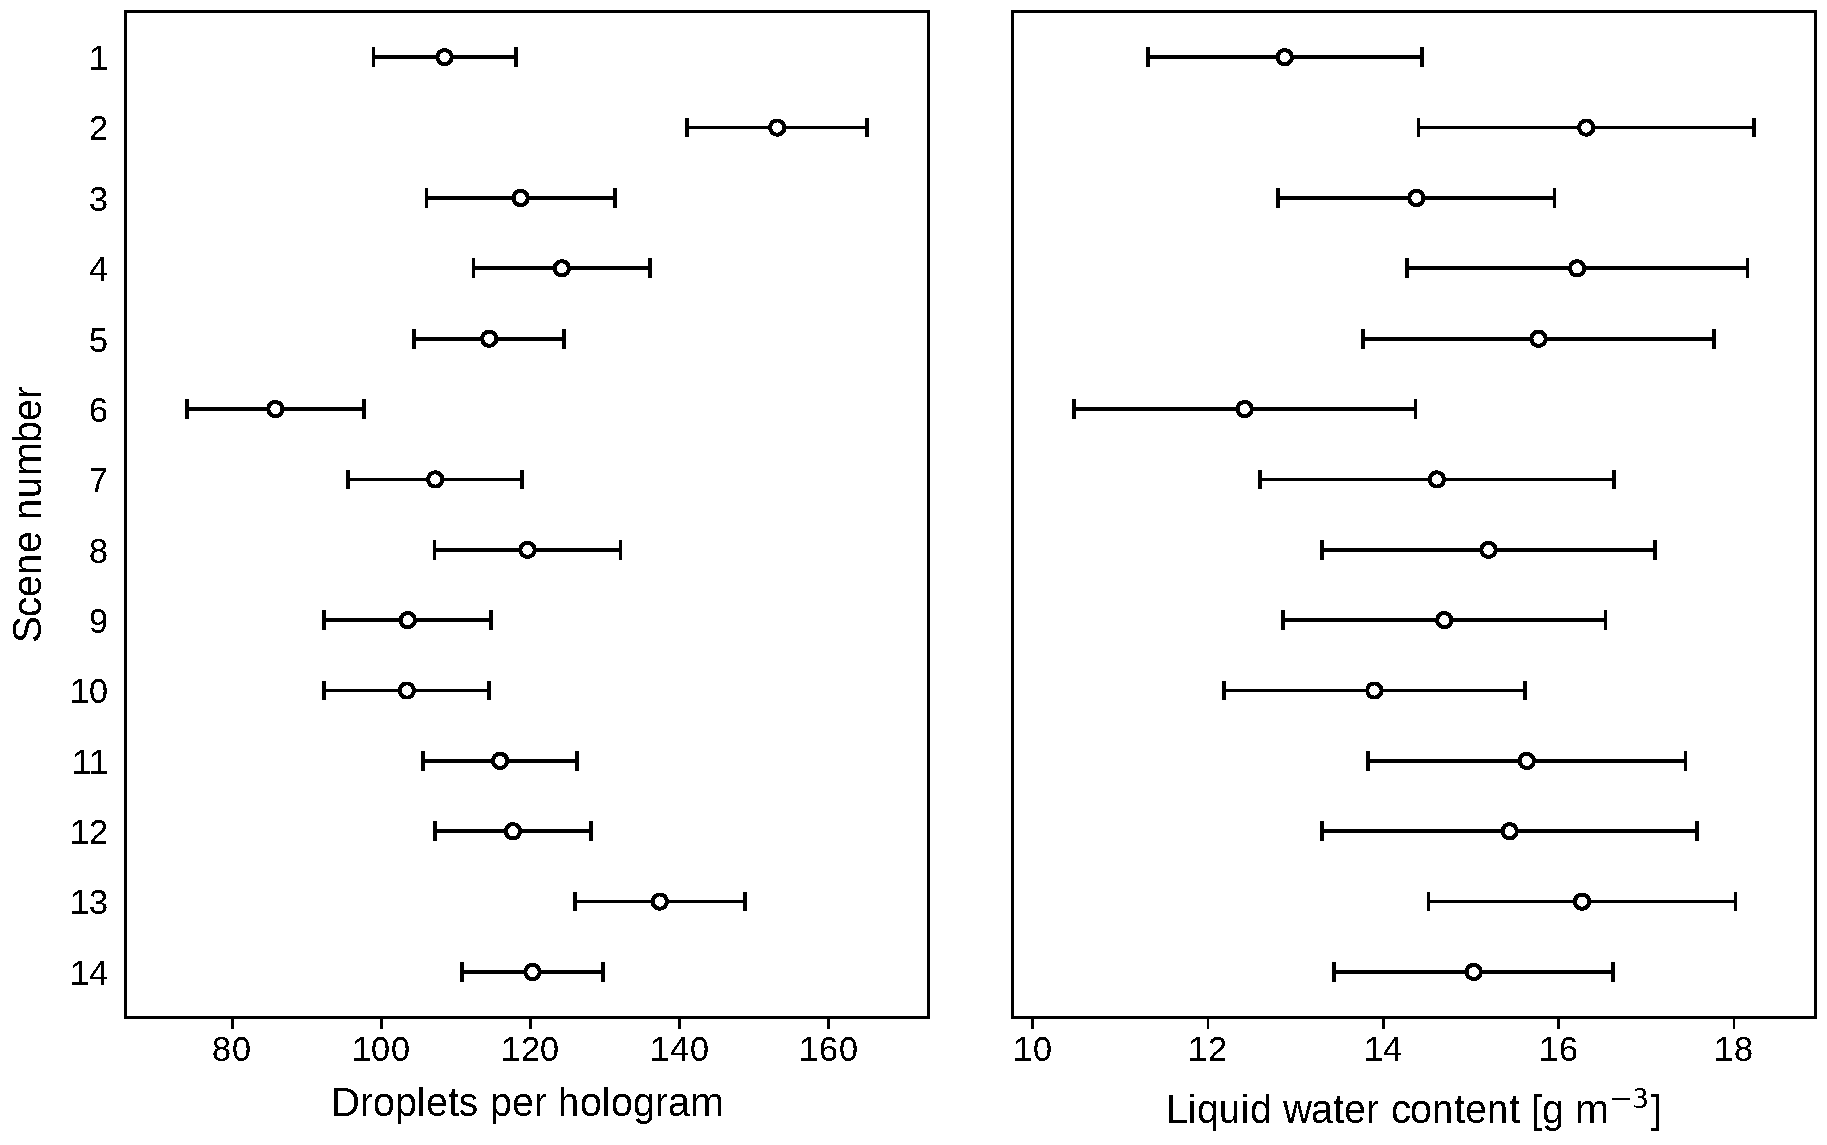
\includegraphics[width=0.98\linewidth]{figures/methods/particle_count_lwc_scene_summary.pdf}
    \subcaption{
      Droplet count per hologram and liquid water content
    }
  \end{minipage}
  \caption{
    Measured droplet population statistics for the 14 experimental sequences. (a) Droplet number-density distribution, \(dn/dD\), as a function of diameter \(D\). The solid curve is the arithmetic mean of the sequence-specific distributions, and the shaded region is the pointwise 95\% confidence interval obtained by resampling the sequences. (b) Droplet count per hologram and liquid water content for each sequence. Symbols indicate the sequence mean, and horizontal error bars indicate the sequence standard deviation.
  }
  \label{fig:exp_data_nd}
\end{figure}


\clearpage
\setcounter{figure}{4}
\begin{figure}
  \centering
  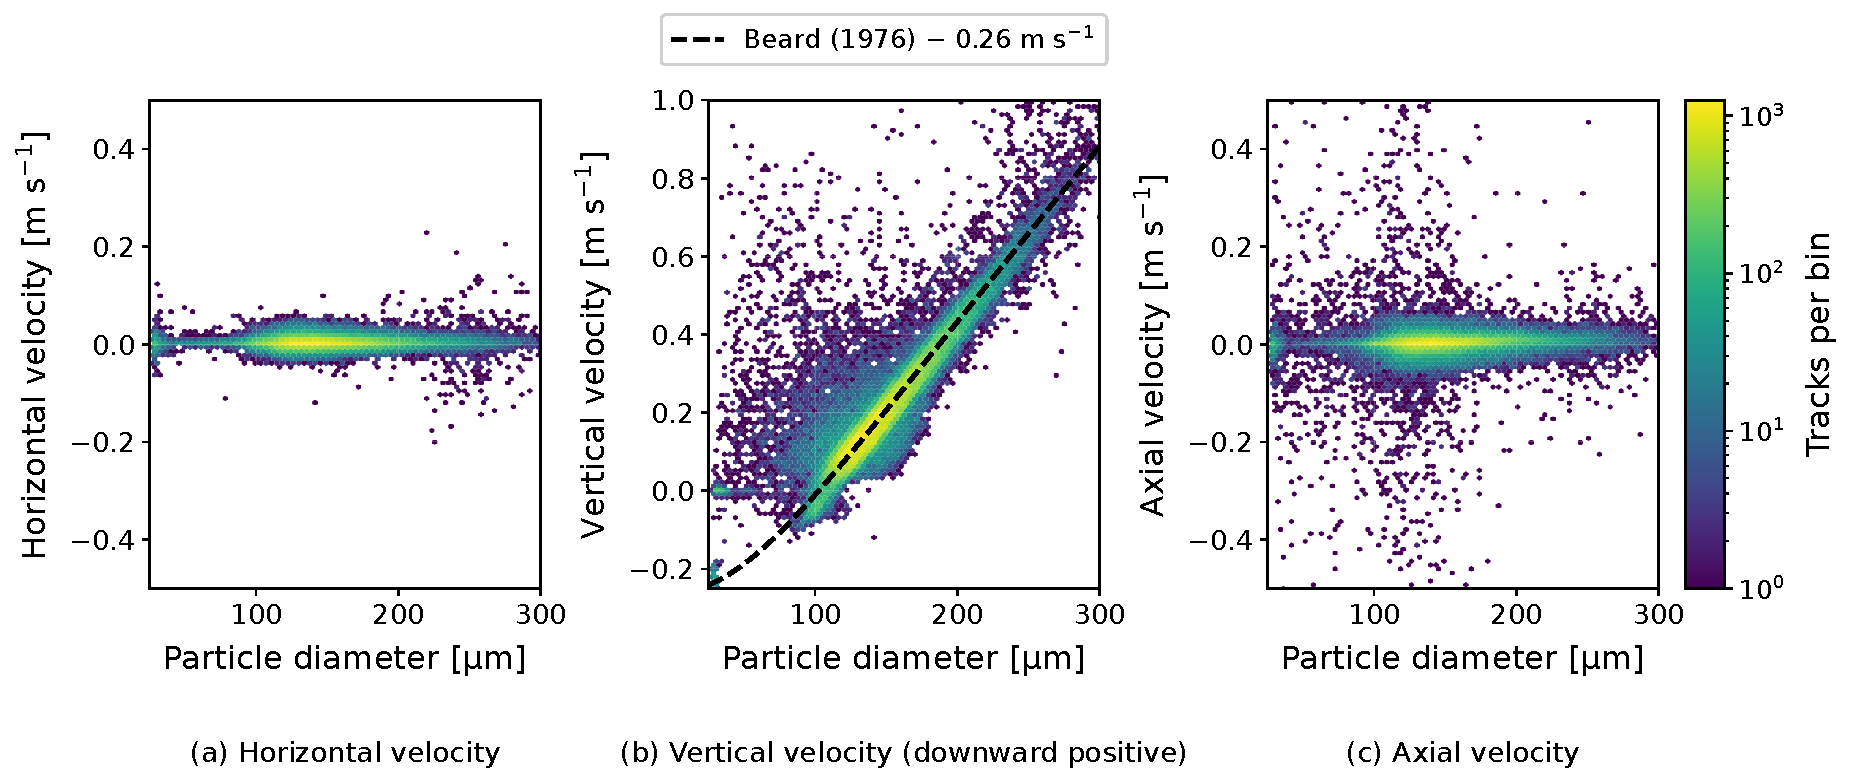
\includegraphics[width=0.98\linewidth]{figures/methods/velocity_distributions_260715.pdf}
  \caption{
    Joint distributions of droplet diameter and velocity obtained from the reconstructed trajectories in the 14 experimental sequences. The panels show the (a) horizontal velocity \(v_x\), (b) vertical velocity \(v_y\), with downward motion defined as positive, and (c) axial velocity \(v_z\), along the optical axis. Color indicates the number of trajectories in each bin on a logarithmic scale. The dashed curve in (b) represents the terminal velocity of Beard (1976), reduced by the mean upward air velocity of \qty{0.26}{\meter\per\second}.
  }
  \label{fig:exp_data_velocity}
\end{figure}


\clearpage
\setcounter{figure}{6}
\begin{figure}[H]
  \begin{subfigure}[t]{0.48\linewidth}
    \centering
    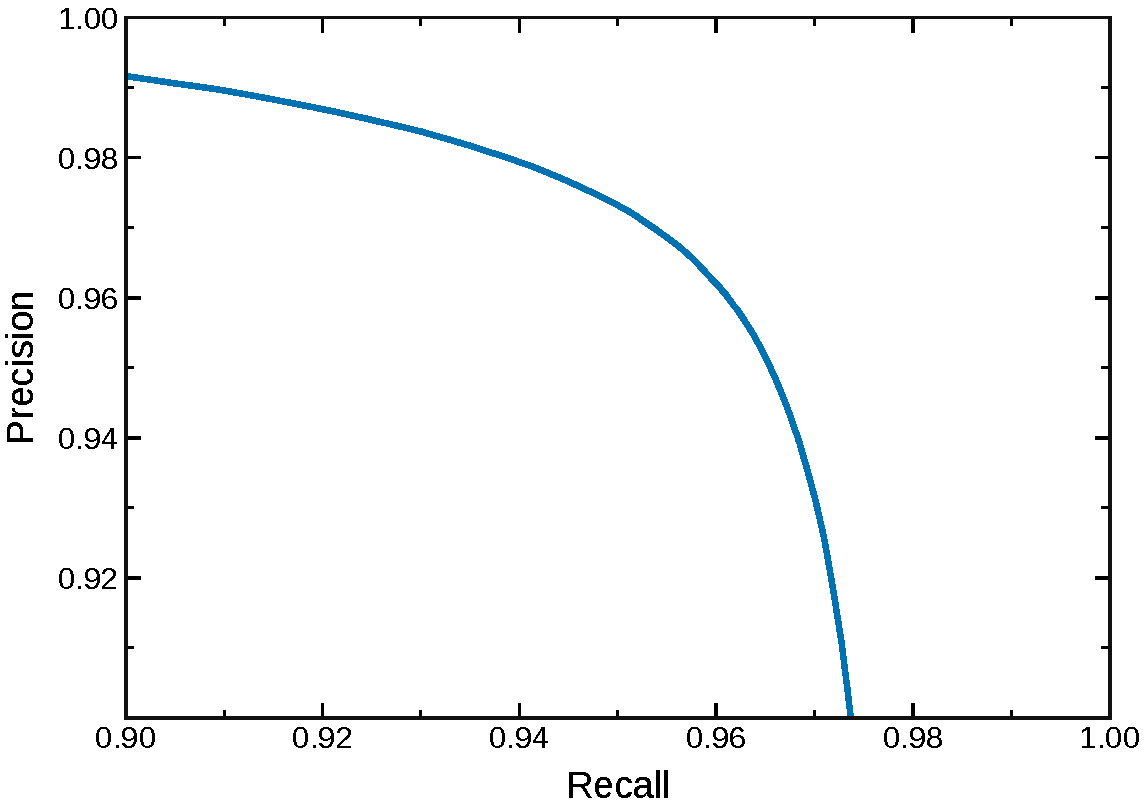
\includegraphics[width=\linewidth]{figures/methods/01_particle_detection_pr_curve_seed260745.pdf}
    \caption{}
  \end{subfigure}
  \hfill
  \begin{subfigure}[t]{0.48\linewidth}
    \centering
    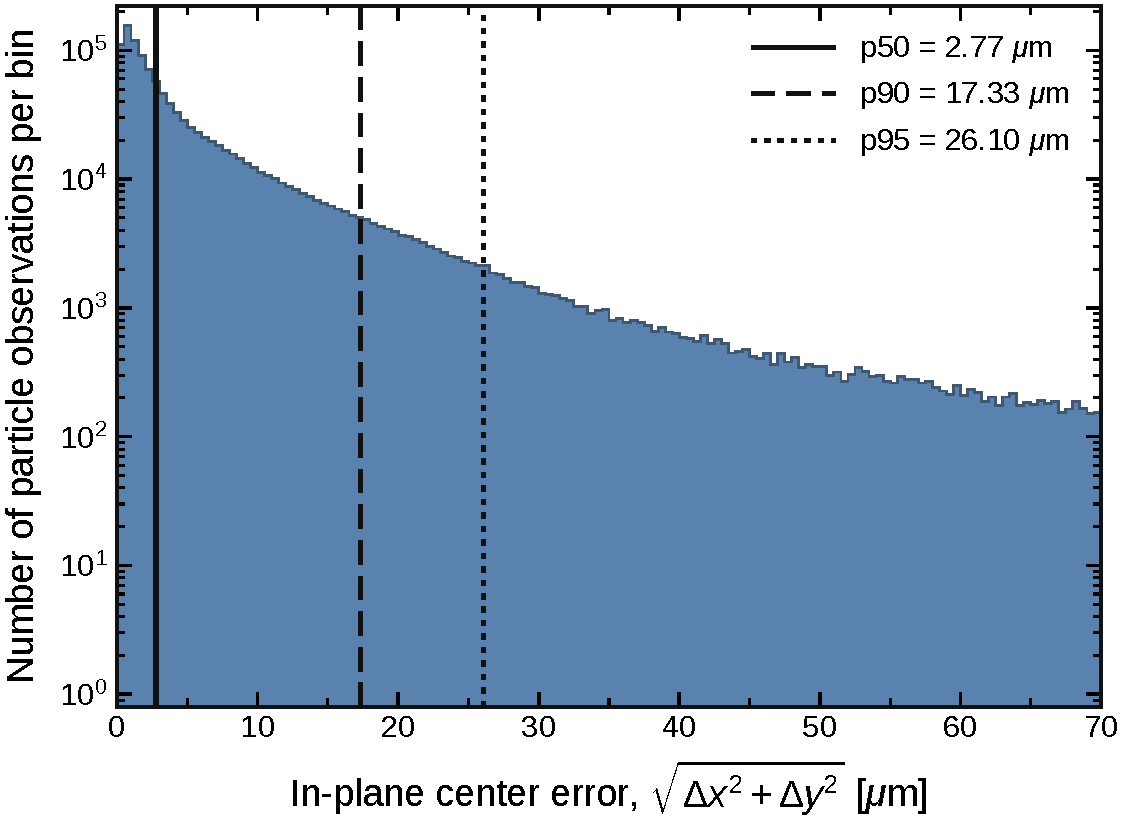
\includegraphics[width=\linewidth]{figures/methods/02_xy_center_error_smoothed_hist_seed260745.pdf}
    \caption{}
  \end{subfigure}

  \medskip

  \begin{subfigure}[t]{0.48\linewidth}
    \centering
    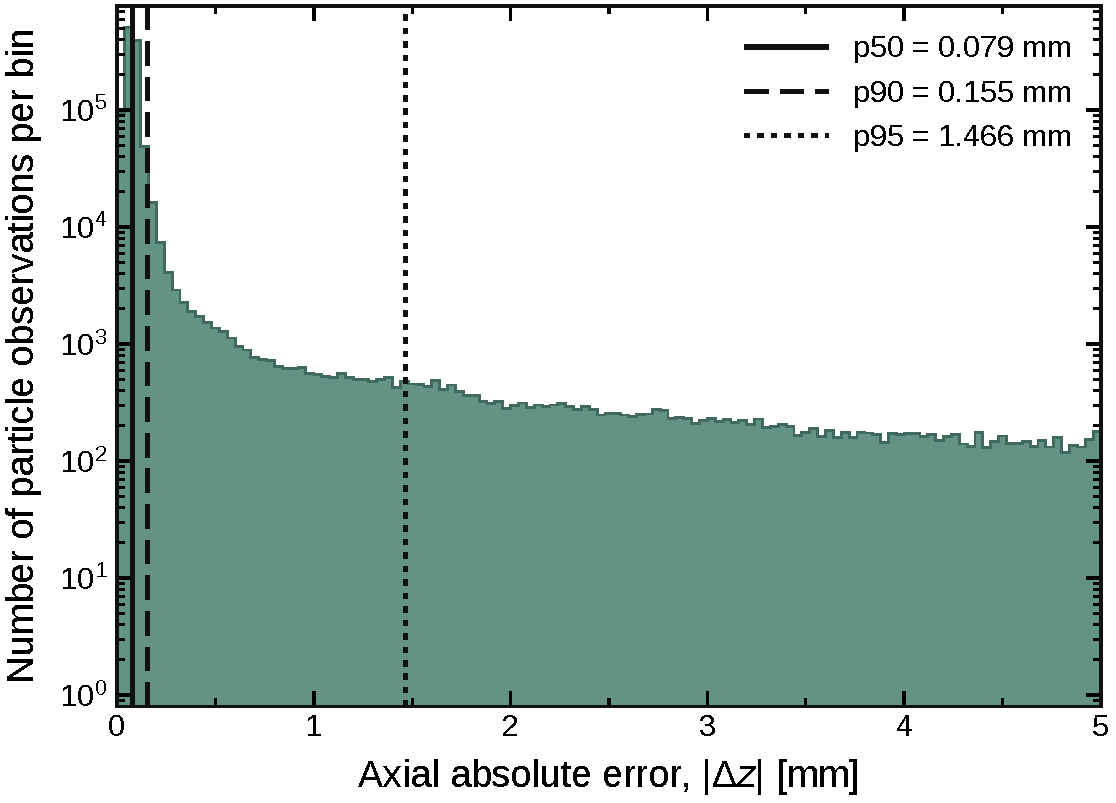
\includegraphics[width=\linewidth]{figures/methods/03_axial_error_smoothed_hist_seed260745.pdf}
    \caption{}
  \end{subfigure}
  \hfill
  \begin{subfigure}[t]{0.48\linewidth}
    \centering
    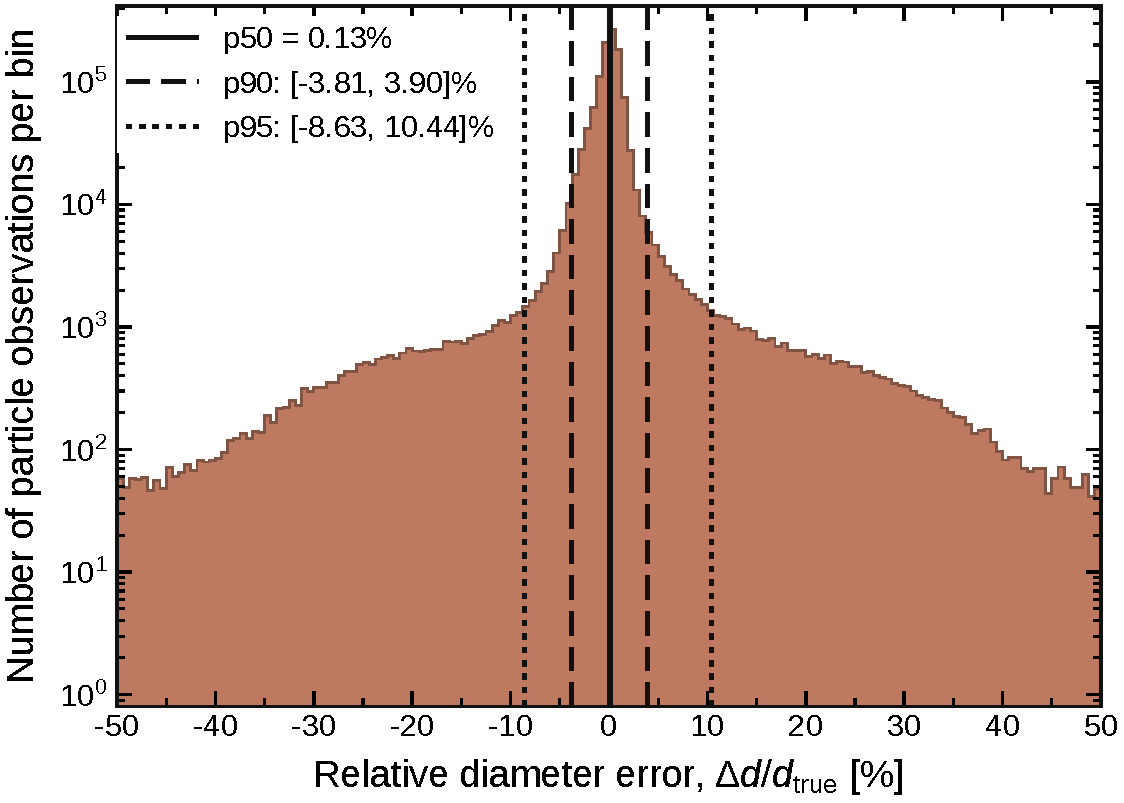
\includegraphics[width=\linewidth]{figures/methods/04_diameter_relative_error_hist_seed260745.pdf}
    \caption{}
  \end{subfigure}

  \medskip

  \begin{subfigure}[t]{0.48\linewidth}
    \centering
    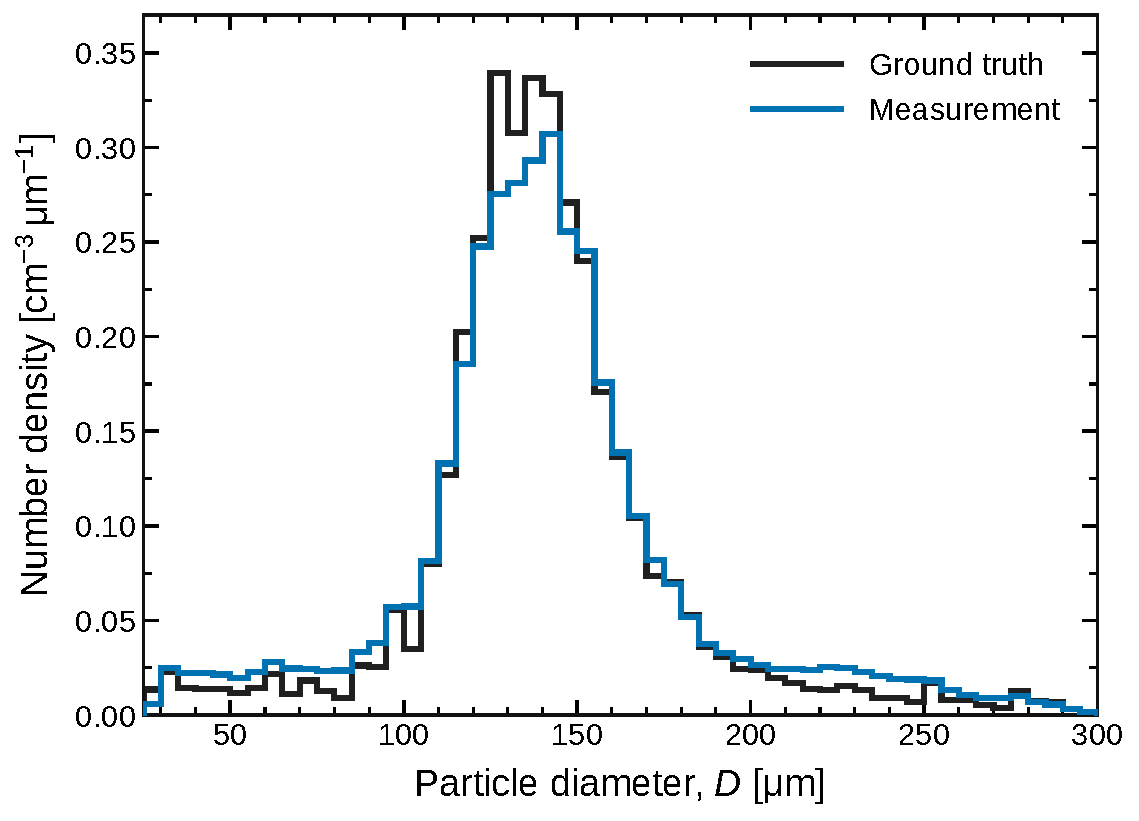
\includegraphics[width=\linewidth]{figures/methods/paper_number_density_distribution_25_300um_seed260745.pdf}
    \caption{}
  \end{subfigure}
  \hfill
  \begin{subfigure}[t]{0.48\linewidth}
    \centering
    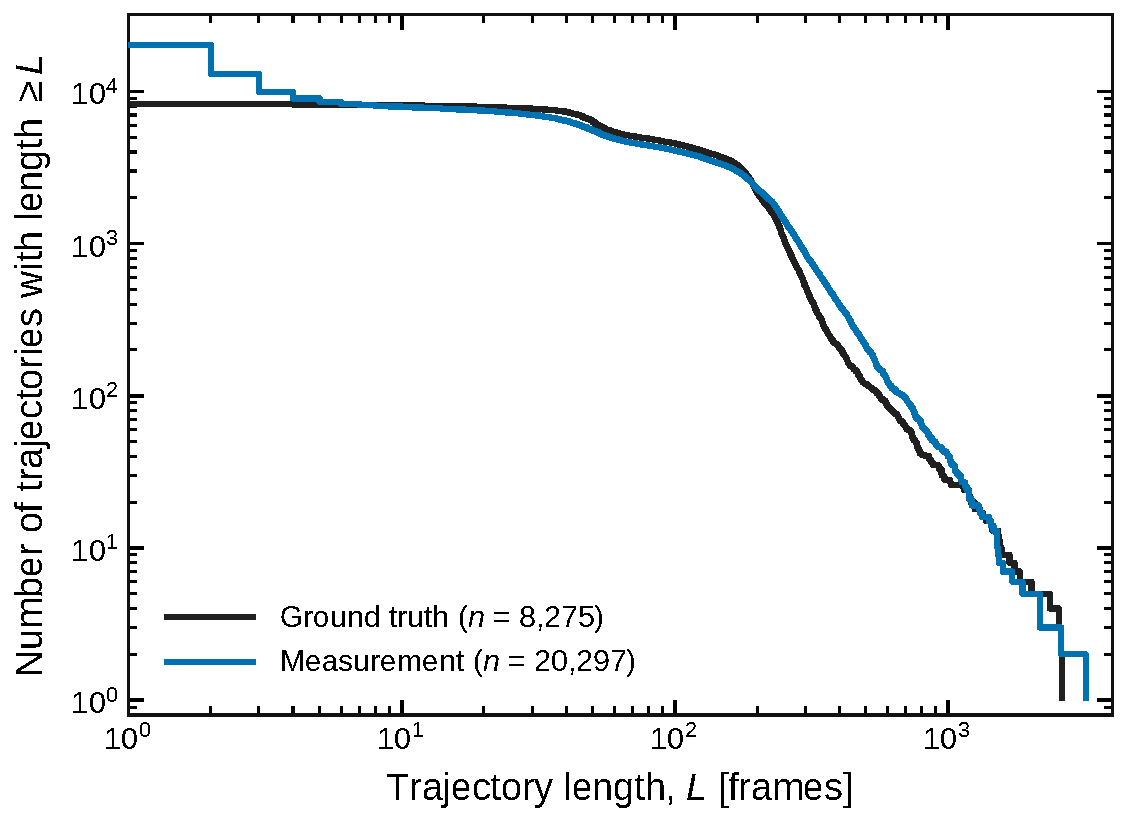
\includegraphics[width=\linewidth]{figures/methods/paper_trajectory_length_counts_25_300um_seed260745.pdf}
    \caption{}
  \end{subfigure}
  \caption{Performance of holographic droplet detection and tracking using HoloD3\cite{HoloD3} on the synthetic test sequence. (a) Particle-level precision--recall curve. Histograms show (b) the in-plane position error, \(\sqrt{\Delta x^2+\Delta y^2}\), (c) the absolute axial-position error, \(|\Delta z|\), and (d) the signed relative diameter error, \(100(D_{\mathrm{meas}}-D_{\mathrm{true}})/D_{\mathrm{true}}\). Annotations in (b,c) report the 50th, 90th, and 95th percentiles; those in (d) report the median and central 90\% and 95\% intervals. (e) Ground-truth and measured number-density distributions. (f) Cumulative numbers of trajectories with length greater than or equal to \(L\), for the ground-truth and reconstructed trajectories.}
  \label{fig:synthetic_hologram_distribution}
\end{figure}


\clearpage
\setcounter{table}{2}
\begin{table}[tbp]
  \centering
  \caption{Event-level performance of the proposed method, the depth-free variant using MinIP image features, and MinIP-based 2D on the synthetic test sequence. Events are matched one-to-one within the common spatiotemporal gate defined by in-plane distance and time difference in Sec.~\ref{sec:synthetic_hologram_generation}. Average precision summarizes the precision-recall curve, and the maximum F1 score is obtained by varying the score threshold. Precision is additionally reported at target recalls of 0.8 and 0.9. Candidate-pool recall is evaluated for the generated candidate pool $\mathcal{H}$, before candidate-wise scoring and duplicate suppression. Values in parentheses denote the difference from Ours (method minus Ours).}
  \label{tab:projected_xy_metric_summary}
  \begin{tabular}{lrrr}
    \hhline{====}
    Metric & Ours & \shortstack{Depth-free\\variant} & \shortstack{MinIP-based\\2D} \\
    \hline
    Average Precision & 0.917 & 0.901 ($-0.016$) & 0.858 ($-0.059$) \\
    Maximum $F_1$ & 0.878 & 0.846 ($-0.032$) & 0.811 ($-0.067$) \\
    Precision at recall $=0.8$ & 0.960 & 0.895 ($-0.065$) & 0.813 ($-0.147$) \\
    Precision at recall $=0.9$ & 0.766 & 0.637 ($-0.129$) & 0.424 ($-0.342$) \\
    Candidate-pool recall & 0.985 & 0.990 ($+0.005$) & 0.991 ($+0.006$) \\
    \hhline{====}
  \end{tabular}
\end{table}


\clearpage
\setcounter{figure}{7}
\begin{figure}[H]
  \centering
  \begin{subfigure}[t]{0.48\linewidth}
    \centering
    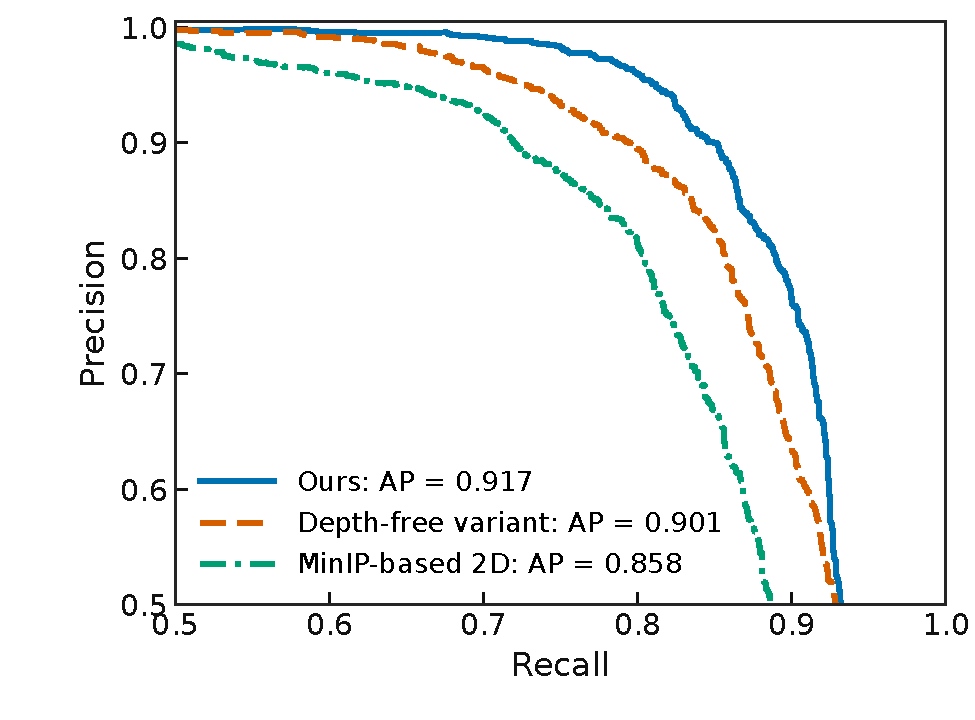
\includegraphics[width=\linewidth]{figures/synthresult/01_validation_precision_recall.pdf}
    \caption{}
    \label{fig:synthetic_hologram_validation_results_pr_curve}
  \end{subfigure}
  \hfill
  \begin{subfigure}[t]{0.48\linewidth}
    \centering
    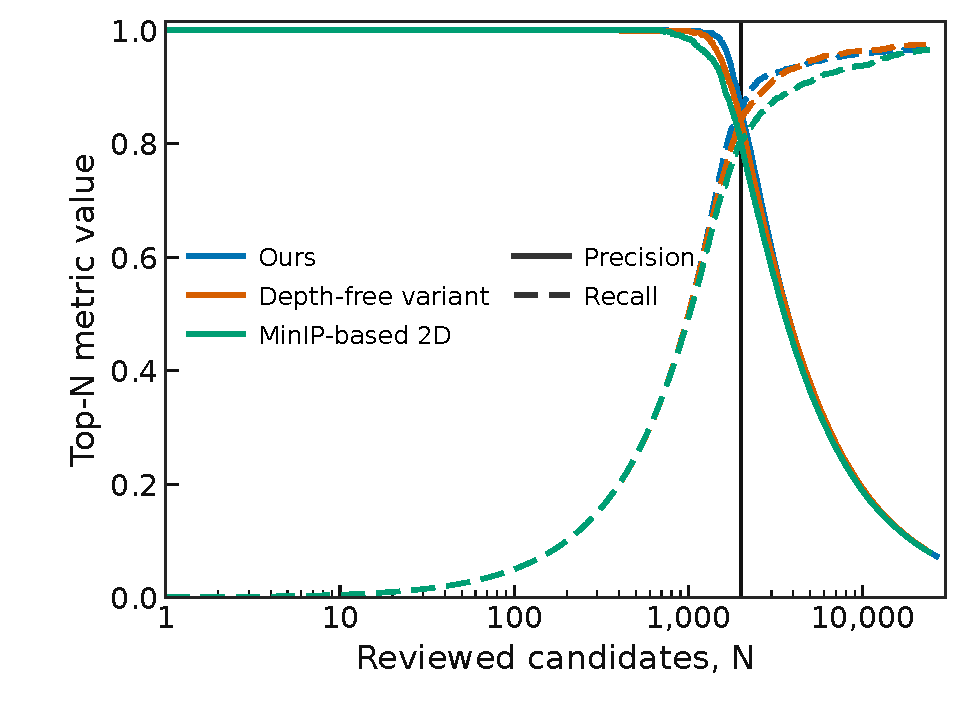
\includegraphics[width=\linewidth]{figures/synthresult/02_validation_topn_precision_recall.pdf}
    \caption{}
    \label{fig:synthetic_hologram_validation_results_topn}
  \end{subfigure}

  \medskip
  \begin{subfigure}[t]{0.48\linewidth}
    \centering
    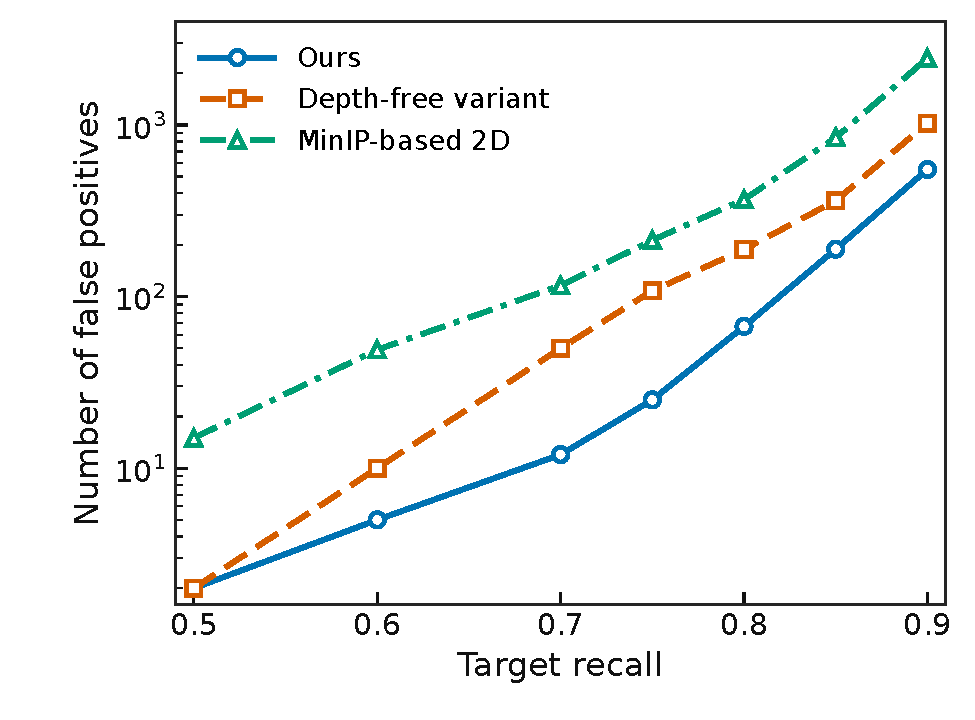
\includegraphics[width=\linewidth]{figures/synthresult/03_validation_false_positive_burden.pdf}
    \caption{}
    \label{fig:synthetic_hologram_validation_results_fp_burden}
  \end{subfigure}
  \hfill
  \begin{subfigure}[t]{0.48\linewidth}
    \centering
    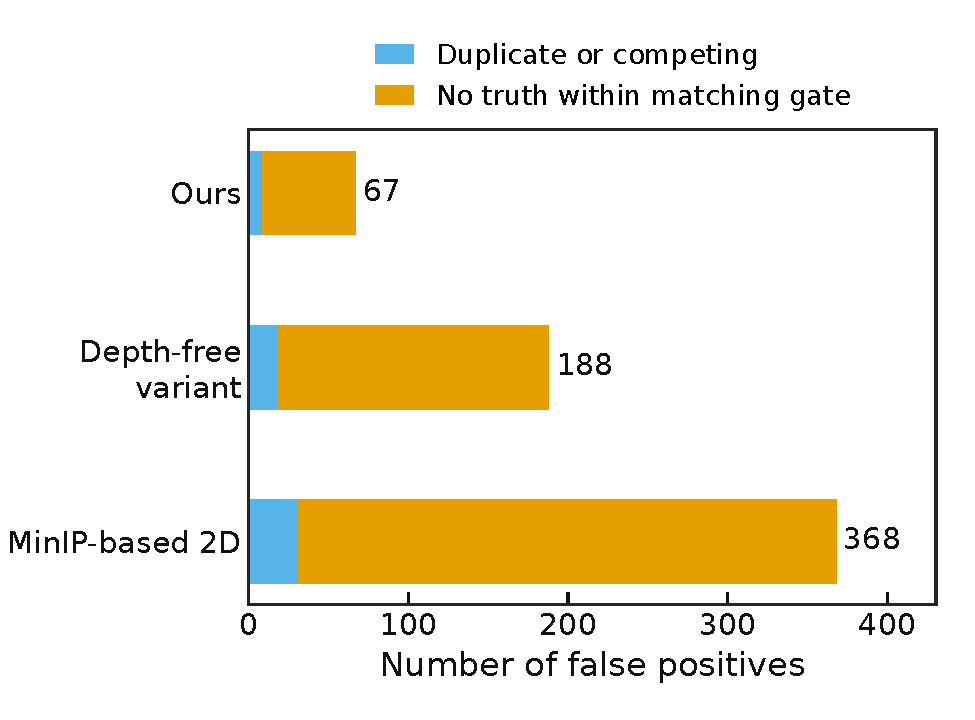
\includegraphics[width=\linewidth]{figures/synthresult/04_validation_false_positive_composition.pdf}
    \caption{}
    \label{fig:synthetic_hologram_validation_results_fp_composition}
  \end{subfigure}
  \caption{Event-detection performance and review burden on the synthetic test sequence containing 2,000 ground-truth events. The proposed method is compared with a depth-free variant using the same measured trajectories and MinIP image features, and with MinIP-based 2D. (a) Event-level precision--recall curves. (b) Precision (solid lines) and recall (dashed lines) among the top \(N\) ranked candidates. (c) Number of false-positive candidates at each target recall. (d) False-positive composition at a target recall of 0.8, separated into duplicate or competing detections and candidates with no ground-truth event within the matching gate.}
  \label{fig:synthetic_hologram_validation_results}
\end{figure}


\clearpage
\setcounter{table}{3}
\begin{table}[H]
  \centering
  \small
  \caption{
    Cumulative stage ablation on the synthetic test sequence containing 2,000 ground-truth events. Image features, relation-attention, and duplicate suppression are added successively to the trajectory-feature model. At each target recall, precision and false-positive counts are evaluated at the same highest score threshold attaining that recall, including tied scores jointly. AP denotes average precision, P precision, R recall, and FP the number of false positives. Arrows indicate the favorable direction.
  }
  \label{tab:projected_xy_stage_ablation}
  \resizebox{\linewidth}{!}{%
    \begin{tabular}{lrrrrr}
      \toprule
      Variant
        & AP $\uparrow$
        & $P$ at $R\geq0.8$ $\uparrow$
        & FP at $R\geq0.8$ $\downarrow$
        & $P$ at $R\geq0.9$ $\uparrow$
        & FP at $R\geq0.9$ $\downarrow$ \\
      \midrule
      Trajectory features only
        & 0.879
        & 0.857
        & 266
        & 0.532
        & 1,583 \\
      + image features
        & 0.888
        & 0.881
        & 216
        & 0.603
        & 1,186 \\
      + relation-attention
        & 0.896
        & 0.917
        & 144
        & 0.668
        & 896 \\
      + duplicate suppression
        & 0.917
        & 0.960
        & 67
        & 0.766
        & 550 \\
      \bottomrule
    \end{tabular}%
  }
\end{table}


\clearpage
\setcounter{figure}{10}
\begin{figure}[H]
  \centering
  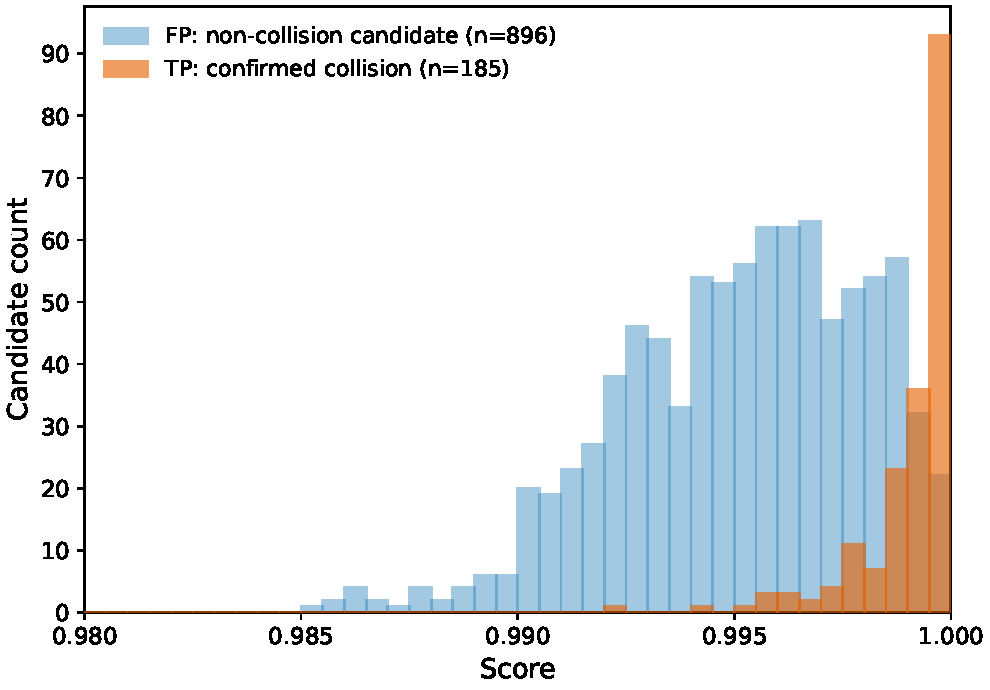
\includegraphics[width=\linewidth]{figures/expresult/review_tp_fp_score_distributions_260715.pdf}
  \caption{Final ranking-score distributions of the 1,081 visually reviewed experimental candidates, excluding ambiguous candidates. The histograms distinguish 185 confirmed collision-coalescence events from 896 rejected candidates. Confirmed events are concentrated toward the upper end of the ranking, although rejected candidates remain in the same score range.}
  \label{fig:experimental_review_score_distribution}
\end{figure}


\clearpage
\setcounter{figure}{11}
\begin{figure}[H]
  \centering
  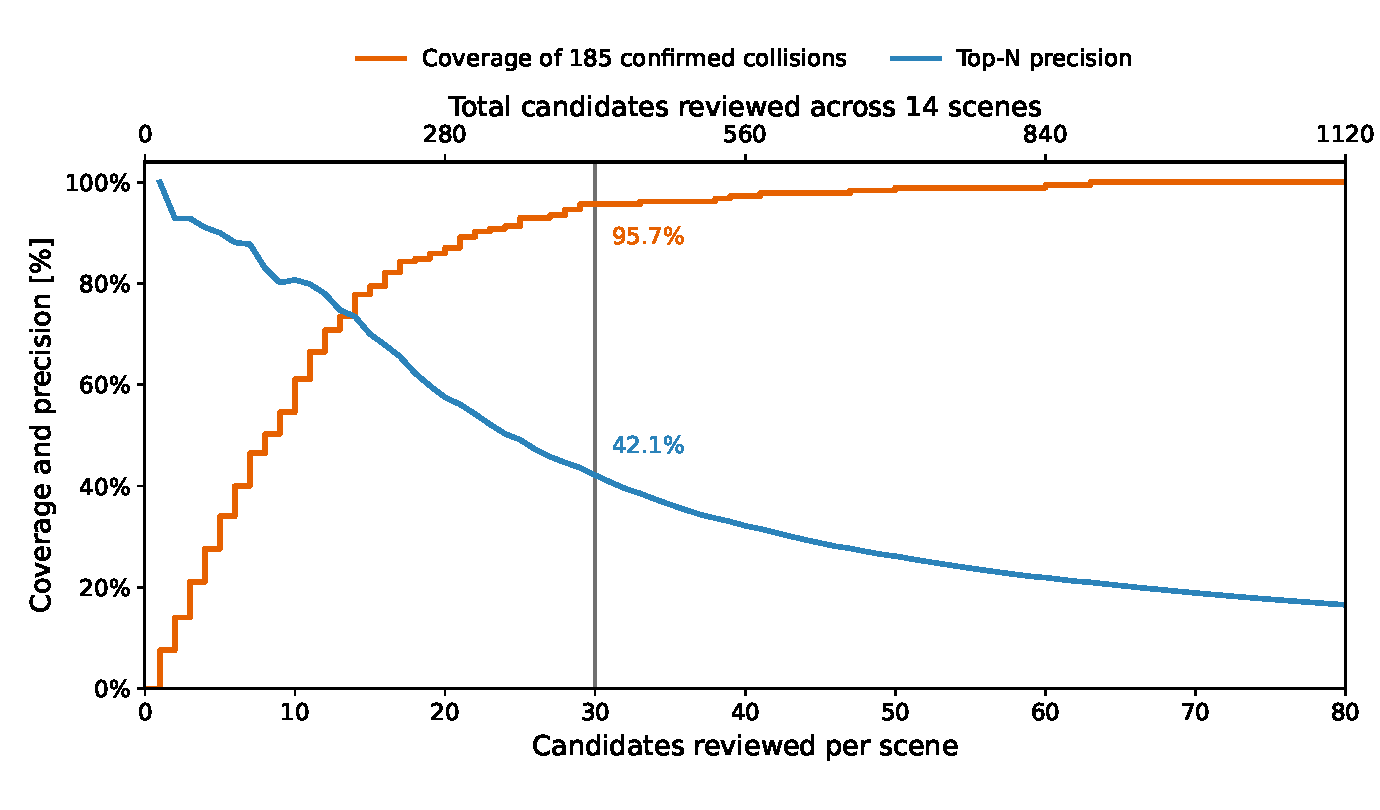
\includegraphics[width=\linewidth]{figures/expresult/review_budget_operating_points_260715.pdf}
  \caption{Coverage of confirmed events and review precision as functions of the number of candidates reviewed per experimental sequence. Candidates are reviewed in descending order of their final score within each of the 14 sequences. Coverage is the fraction of the 185 confirmed events recovered, whereas top-\(N\) precision is the fraction of reviewed candidates confirmed as events. The upper axis gives the total number reviewed across all sequences. Reviewing the top 30 candidates per sequence, or 420 candidates in total, recovers 177 events, corresponding to 95.7\% coverage and 42.1\% precision. Coverage is conditional on the confirmed-event set and is not an estimate of absolute experimental recall.}
  \label{fig:experimental_review_budget_operating_points}
\end{figure}


\clearpage
\setcounter{figure}{12}
\begin{figure}[H]
  \centering
  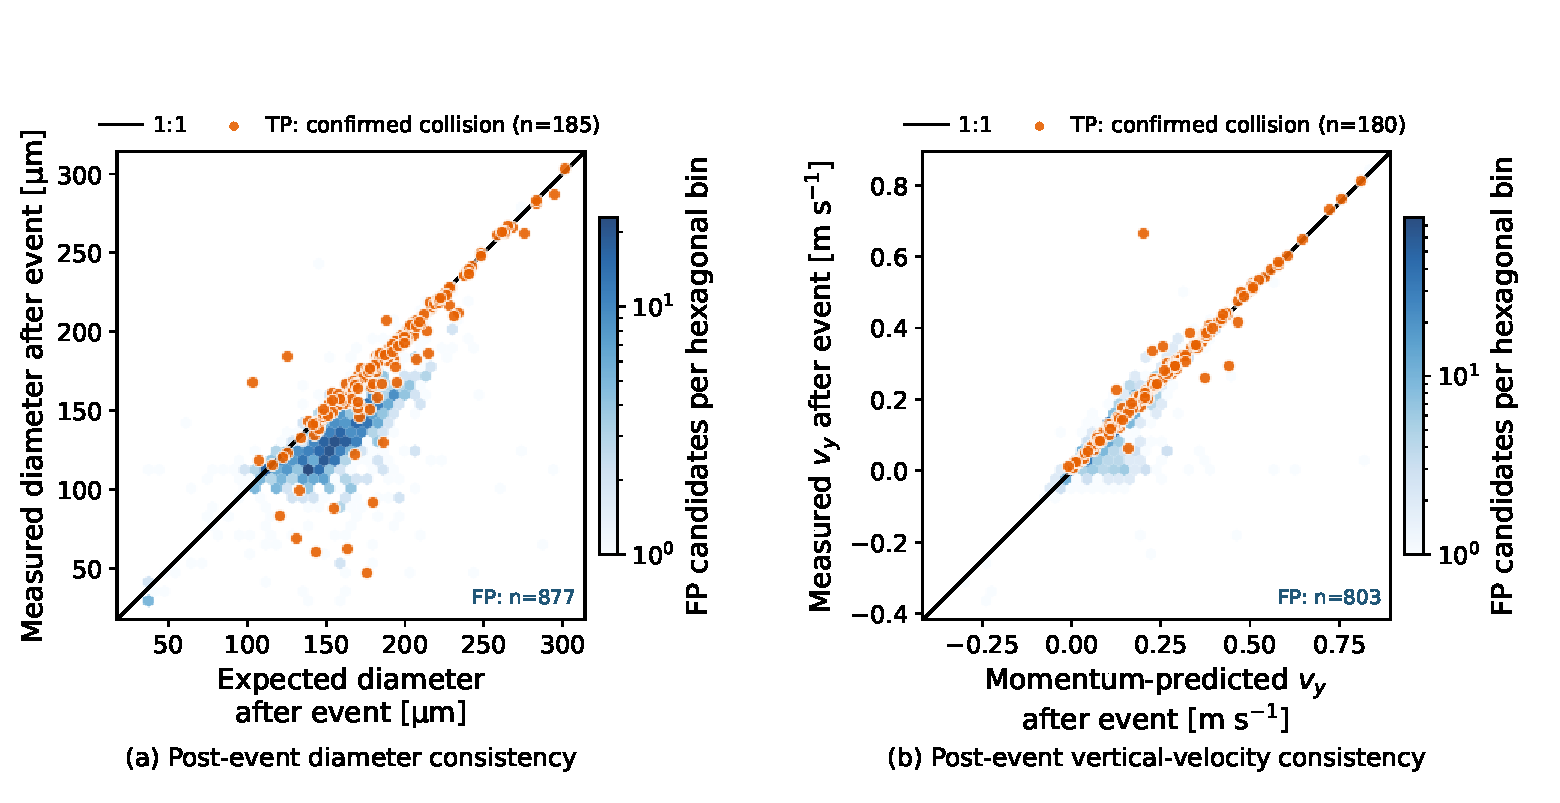
\includegraphics[width=\linewidth]{figures/expresult/physical_consistency_combined_260715.pdf}
  \caption{Physical-consistency diagnostics for visually reviewed experimental candidates. (a) Measured post-event diameter versus the volume-conservation prediction, \(D_{\mathrm{exp}}=(D_1^3+D_2^3)^{1/3}\). (b) Measured post-event vertical velocity versus the momentum-conservation prediction, \(v_{y,\mathrm{exp}}=(D_1^3v_{y,1}+D_2^3v_{y,2})/(D_1^3+D_2^3)\), with downward velocity positive. Orange markers show confirmed events: 185 in (a) and 180 with valid velocity estimates in (b). Blue hexagonal bins show the numbers of rejected candidates on logarithmic color scales. Black lines indicate one-to-one agreement.}
  \label{fig:experimental_physical_consistency}
\end{figure}


\clearpage
\setcounter{figure}{13}
\begin{figure}[H]
  \centering
  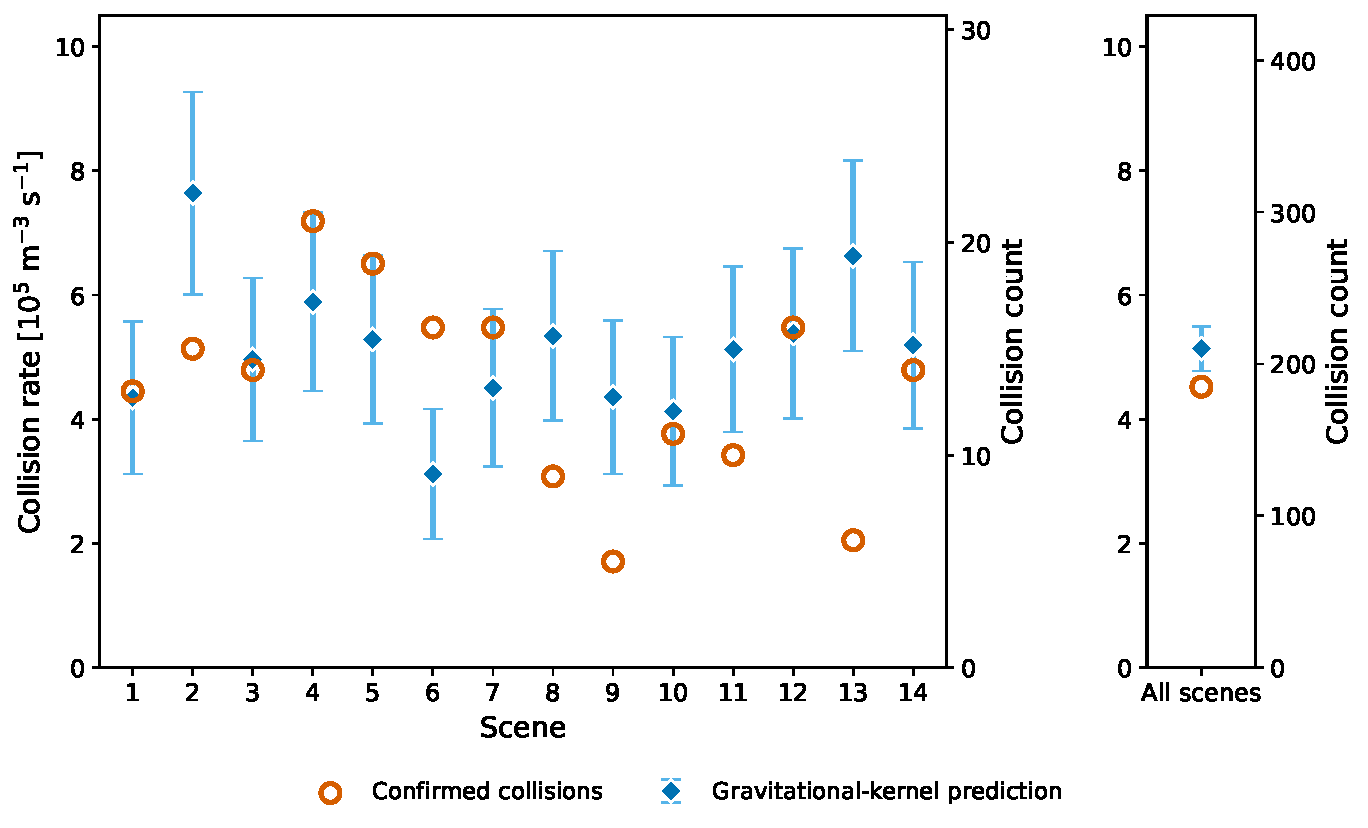
\includegraphics[width=\linewidth]{figures/expresult/scene_collision_counts_observed_vs_hall_260715.pdf}
  \caption{Comparison of confirmed collision–coalescence counts and volumetric collision rates with gravitational-kernel predictions. The left panel shows the 14 experimental sequences separately, and the right panel shows the pooled result. Open circles denote visually confirmed events without correction for missed detections. Filled diamonds denote predictions obtained using the experimentally measured droplet number-density distributions, with error bars indicating ±1 standard deviation as defined in Section \ref{sec:collision_statistics}. The left vertical axes show collision rates per unit volume and time, and the right vertical axes show the corresponding counts for the relevant observation duration.}
  \label{fig:experimental_scene_collision_counts}
\end{figure}


\clearpage
\setcounter{figure}{14}
\begin{figure}[H]
  \centering
  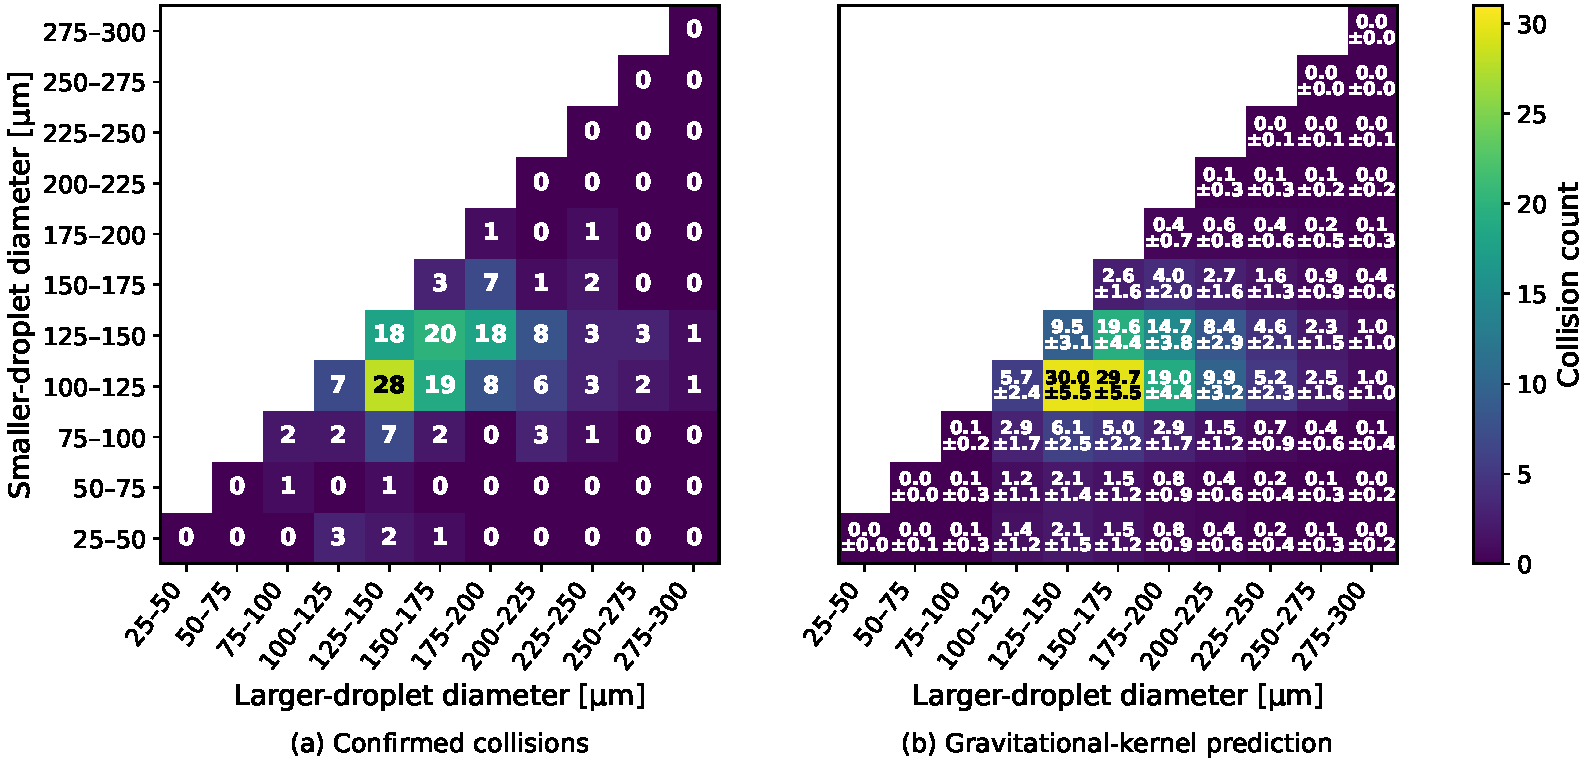
\includegraphics[width=\linewidth]{figures/expresult/collision_count_map_observed_vs_hall_260715.pdf}
  \caption{Parent-diameter-pair distributions of collision–coalescence counts pooled over the 14 experimental sequences. (a) Visually confirmed event counts. (b) Gravitational-kernel predictions using the experimentally measured number-density distributions. The horizontal and vertical axes represent the larger and smaller parent diameters, respectively, using \qty{25}{\micro\meter} bins over \(\qty{25}{\micro\meter}\leq D<\qty{300}{\micro\meter}\). Each unordered diameter-bin pair is counted once. Diagonal cells include droplets in the same diameter bin, not necessarily droplets of identical diameter. Cell annotations in (b) give the predicted count ±1 standard deviation, rounded to one decimal place.}
  \label{fig:experimental_collision_count_map}
\end{figure}

\end{document}
